\chapter{Introduction}
%\addcontentsline{toc}{chapter}{Introduction} 

%\subsection{Motivation}
%\label{subsec:label}

In this first chapter, we introduce the reader to the research context and background of this thesis, situating the work in the research line of our group. Afterwards, we describe the proposed objectives and the respective stages to cover. Finally, we summarize the main structure of this thesis, highlighting the conceptual thread between each of the articles that compose its main core. 

\section{Research context}
\label{sec:introduction_research_context}

\subsection{Multiple Sclerosis}
\label{sub:introduction_multiple_sclerosis}

The human nervous system can be divided into the central nervous system (CNS) consisting of the brain and the spinal chord, and the peripheral nervous system, which connects the CNS with the sense organs \cite{Brodal2010}. CNS is mainly composed of two tissue components: gray matter (GM), which consists of neuronal cell bodies; and white matter tissue (WM), which is mainly composed of myelinated axon tracts \cite{Sperber2006}. The brain itself is composed mostly of GM and WM, both surrounded by the Cerebro-spinal fluid (CSF), which provides basic mechanical and immunological protection to the brain inside the skull \cite{Sperber2006}. 

Multiple sclerosis (MS) is the most common chronic immune-mediated disabling neurological disease of the CNS \cite{Steinman1996}, in which the insulating covers of the nerve cells in the spinal chord and brain are damaged \cite{Compston2008}. Nowadays, MS is the most frequent non-traumatic neurological disease that causes more disability in young adults. It follows a similar behavior to other putative autoimmune diseases, and affects twice as many women as men \cite{Confavreux1980}. It has a low incidence in childhood, but the probability increases rapidly in young adulthood reaching a peak between 25 and 35 years, and then slowly declines, becoming rare at 50 and older \cite{Cabezas2011}. So far, the world estimate for the disease is between 1.3 to 2.5 million cases, being relatively common in Europe, the United States, Canada, New Zealand, and parts of Australia, but rare in Asia, and in the tropics and subtropics \cite{Cabezas2011}. 

MS is characterized by areas of inflammation, demyelination, axonal loss, and gliosis scattered throughout the CNS, often causing motor, sensorial, vision, coordination, deambulation, and cognitive impairment \cite{Compston2002}. Demyelination is the process of progressive damage to the protective covering (myelin sheat) around the axon of the neurons. Demyelinated axons conduct impulses at reduced or spontaneous velocity causing impairment in sensation, movement and cognition \cite{Compston2008}. The different clinical courses of the disease are generally grouped into four subtype forms \cite{Lublin1996}. The  \textit{Relapsing/Remitting} (RRMS) form of the disease is characterized by exacerbation times where symptoms are present. These periods are followed by periods of remission, where the patient recovers partially or totally from the disease's symptoms. The \textit{Secondary Progressive} (SPMS) form is characterized by a gradual intensification of symptoms between affection relapses. The \textit{Progressive remitting} (PRMS) form is typified by an increase in the relapse times with significant recovery but with worsening symptoms in new relapse intervals. Lastly, the \textit{Primary Progressive} (PPMS) form is characterized by a severe decrease of remission times with special localization in the brain. In general, 50\% of RRMS patients develop the SPMS form of the disease after 10 years. After 25 years, 90\% of RRMS patients will develop the SPMS form \cite{Lublin1996}.


%MRI images are created by computing mathematical inverse transformations of the energy released by hydrogen ions being exposed to different magnetic fields and radio waves. 
\subsection{Magnetic Resonance Imaging in MS}
\label{subsec:introduction_magnetic_resonance_imaging}
Magnetic Resonance Imaging (MRI) is a noninvasive medical imaging technique  used in radiology to generate image representations of different internal anatomical organs and physiological processes of the body. Over the last 40 years, MRI has evolved as a clinical modality \cite{Geva2006}, and, in particular, as an essential tool for the diagnosis and evaluation of central nervous system disorders such as MS \cite{Edelman1993}. In MRI, MS plaques are well-delimited regions with hypointense signal intensity with respect to GM on T1-weighted (T1-w), while hyperintense with respect to GM on T2-weighted (T2-w), Proton Density-weighted (PD-w) and Fluid Attenuated Inversion Recovery (FLAIR) modalities (see Figure \ref{mri_modalities}).

\begin{figure*}[top]
  \begin{center}
    %\vspace{-3cm}
    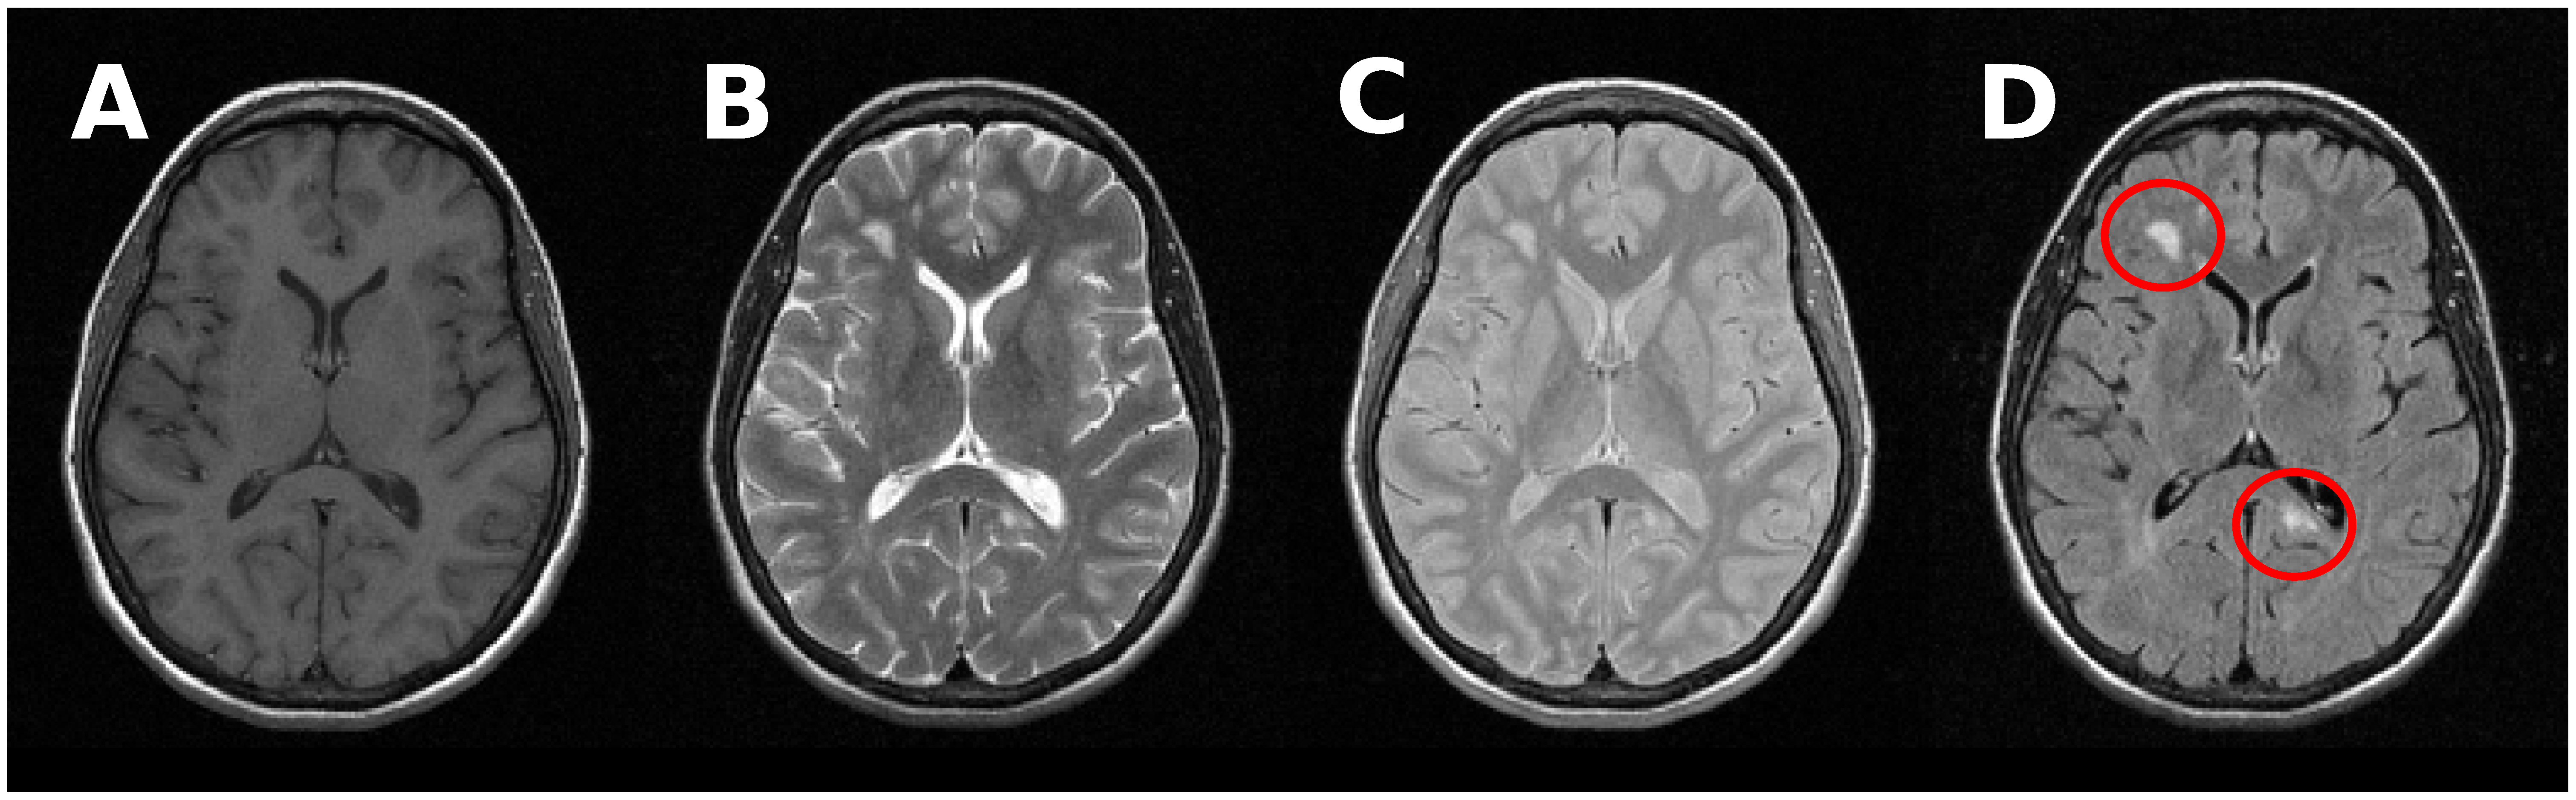
\includegraphics[width=1\textwidth]{figures/figure_1.eps}
  \end{center}
    \caption[MRI image modalities]{MRI image modalities. A) T1-weighted (T1-w) image sequence. B) T2-weighted (T2-w) image sequence. C) Proton Density-weighted (PD-w) image sequence. D) Fluid Attenuated Inversion Recovery (FLAIR) sequence. MS plaques are shown inside red circles on the FLAIR modality. MS plaques are hypointense with respect to GM and WM in T2-w, PD-w and FLAIR sequences, while hypointense with respect to WM on the T1-w modality.}
    \label{mri_modalities}
\end{figure*}

In this aspect, new criteria for MS diagnosis and monitoring has been revised over the last years \cite{Polman2011}, due to MRI sensitivity in showing focal white matter (WM) lesions and disease activity in time and space \cite{Filippi2011}. Additionally, various studies have analyzed the correlation between MRI brain tissue atrophy measurements and MS disability status, showing that tissue loss is an important indication of the disease's progression \cite{Chard2002, Filippi2013, Fisher2008, Rudick2009}. Tissue loss seems to increase through the course of MS at a similar rate between 0.3\% and 0.5\% per year, independently of the MS subtype \cite{DeStefano2010, Rudick2009}. In general, GM atrophy is associated more with disability changes than with WM atrophy \cite{Fisniku2008}, not only in the RRMS and SPMS MS subtypes \cite{Fisher2008, Rudick2009}, but also in Clinically Isolated Syndrome (CIS) patients, where several studies have shown significantly greater ventricular cavities and an associated GM loss in MRI scans of CIS patients that will develop MS compared to those who will not \cite{Ceccarelli2010,Filippi2013}.

\subsection{Image analysis in MS}
\label{subsec:image_analysis}

Manual analysis of brain images is unfeasible in practice, given the large number of two-dimensional slices of each three-dimensional MRI patient image and the possible intra/inter observer variability between experts \cite{Cabezas2011}. This has led to the development since the early nineties of a wide number of lesion and tissue segmentation methods, with the aim of reducing the time needed for  manual interaction and the inherent variability of manual annotations \cite{Cline1990, Gerig1992, Kapur1996}. 


\subsubsection{Pre-processing of MRI images}
Acquired brain MRI volumes incorporate non-brain tissue parts of the head such as eyes, fat, spinal cord or the skull. Brain tissue extraction from non-brain tissue is commonly referred in the literature as skull-stripping (see Figure \ref{preprocessing_mri} B and C). Skull-stripping has a direct effect on the performance of automated methods, as differences in skull stripping would lead to unexpected results in the tissue classification if the skull or eyes were included as brain tissue \cite{Acosta-Cabronero2008, Popescu2012}. Among the different methods proposed for skull-stripping \cite{Acosta-Cabronero2008, Lee2003, Roura2014}, the Brain Extraction Tool (BET) \cite{Smith2002} and the Brain Surface Extractor (BSE) \cite{Shattuck2001} are the most commonly used methods by the neuroimaging community.

Furthermore, inherent characteristics of the MRI acquisition process such as differences in the magnetic field, bandwidth filtering of the data or eddy currents driven by field gradients usually result in image artifacts that may also have a negative impact on the performance of the methods \cite{Simmons1994}. In these cases, intensity correction of the MRI images is performed either before lesion/tissue segmentation, or as an integrated part of the tissue segmentation pipeline  (see Figure \ref{preprocessing_mri} D). Among the formerly available strategies proposed \cite{Arnold2001,Hou2006}, the N3 \cite{Sled1998} and N4 \cite{Tustison2010} methods are currently the most widely used tools used for intensity correction. 


\begin{figure*}[top]
  \begin{center}
    %\vspace{-3cm}
    \includegraphics[width=1.0\textwidth]{figures/figure_2.eps}
  \end{center}
    \caption[MRI pre-processing steps]{MRI pre-processing steps. A) T1-weighted (T1-w) image sequence. B) Computed brain mask using the BET approach \cite{Smith2002} and C) skull stripped T1-w sequence  . D) Estimated T1-w bias-field using the N3 method proposed by \cite{Sled1998}.}
    \label{preprocessing_mri}
\end{figure*}

\subsubsection{Automated lesion segmentation}

MRI based diagnostic criteria for MS has led to an increasing need to analyze focal MS lesions quantitatively in individual and temporal studies \cite{Cabezas2014, Polman2011}. Different sequences such as, T2-w, PD-w and FLAIR, are often used in lesion detection and segmentation, as MS lesions appear brighter than GM and WM in them. However, WM lesions often present a similar signal intensity profile to CSF in T2-w. In contrast, FLAIR sequences suppress fluids from the image, restraining the CSF tissue effects on the acquired image, although some severe T2-w hyperintense lesions appear similar to CSF in FLAIR \cite{Harmouche2015}. 

A wide number of automated lesion segmentation techniques have been proposed over the last few years \cite{Garcia-Lorenzo2013, Llado2012}. In these methods, lesion segmentation is based either on supervised or unsupervised strategies. Supervised methods employ a training set of correctly-identified observations that are used as prior information to learn the lesion's characteristics. Newer proposed strategies integrate a spatial decision forest \cite{Geremia2011}, statistical methods \cite{Sweeney2013}, patch-based models \cite{Guizard2015} or adaptive dictionary learning strategies \cite{Deshpande2015}. In contrast, unsupervised learning methods do not use any prior information in the segmentation task, which involves grouping data into categories based on some measure of inherent similarity or distance characteristics of the input images. Among these, most recent methods include probabilistic models that separate WM lesions from normal-appearing tissue by considering lesions as an outlier class \cite{Harmouche2015,Jain2015,Tomas-Fernandez2015}, or techniques that make use of the signal intensity of lesions on FLAIR to apply several thresholding methods with post-processing steps to automatically segment lesions \cite{Roura2015, Schmidt2012}. 


\subsubsection{Automated brain tissue segmentation in MS}
\label{subsec:lesion_segmentation}
The correlation between brain tissue atrophy measurements and MS disability status \cite{Filippi2013, Fisher2008} has increased the necessity of developing robust automated brain tissue segmentation methods capable of measuring brain tissue volume accurately \cite{Giorgio2013}. However, the automated segmentation of brain tissue is still a challenging problem due to the complexity of the images, the existence of lesions, differences in tissue intensities, noise, intensity inhomogeneities and the absence of anatomy models that fully capture the deformations possible in each structure \cite{Cabezas2011, Kapur1996}. 

A wide number of brain tissue segmentation methods have been proposed so far. General purpose intensity based methods usually perform tissue segmentation on T1-w sequences, as this modality clearly separates gray matter from white. These include probabilistic strategies based on Bayesian inference \cite{Ashburner2005,Marroquin2002, Roy2012,Shattuck2001}, Markov Random Fields models \cite{Bricq2008, Tohka2010, Zhang2001}, or unsupervised clustering methods \cite{Caldairou2011, Pham2001}. In contrast, supervised learning approaches also combine T1-w sequences with other modalities such as T2-w and PD-w using \textit{K-Nearest-Neighbor} classifiers \cite{deBoer2009,Vrooman2013}, \textit{Support Vector Machines} \cite{Akselrod2006,Opbroek2013}, \textit{Random Forests} \cite{yi2009,Mahapatra2014}, or trained \textit{Gaussian mixture models} \cite{Rajchl2015}. 

However, different studies have shown that tissue abnormalities found in MS patients images such as WM lesions reduce the accuracy of tissue segmentation methods \cite{Battaglini2012, Chard2010}. Effectively, WM lesions on T1-w are hypointense with respect to normal-appearing WM, and  therefore, lesion voxels that are classified as GM distort the overall GM volume. However, lesion voxels may also have an effect on the differences observed in normal-appearing tissue. WM lesions that are actually classified as WM decrease the mean overall signal intensity of the WM, causing GM voxels with signal intensities similar to WM lesions to be also miss-classified as WM.  In contrast, if WM lesions are classified as GM, normal-appearing WM voxels with signal intensities similar to lesions may be miss-classified as GM. 
 
\subsubsection{Lesion filling}
\label{subsec:lesion_filling}
In MS, hypointense WM lesions have to be pre-processed before tissue segmentation in order to reduce the effects of WM lesions on the segmentation. Historically, WM lesions have been masked-out of the T1-w before segmentation, and their volume added to the WM afterwards \cite{Chard2002}. Although this method effectively reduces the error in tissue volume, it has been shown in several studies that this approach is not optimal \cite{Battaglini2012, Chard2010}. 

In this respect, several strategies have proposed in-painting lesions on the T1-w with signal intensities of the normal-appearing WM before tissue segmentation \cite{Battaglini2012, Chard2010, Magon2014, Sdika2009}, a process known in the literature as lesion filling (see Figure \ref{lesion_filling} for an example). However, most of the available lesion filling methods require manual delineations of lesions, which may be a tedious, challenging and time-consuming task depending on the characteristics of the image \cite{Llado2012}. When available, lesion filling has demonstrated  a significant reduction not only in the associated errors of WM lesions in tissue volume measurements \cite{Popescu2014}, but also in image registration \cite{Ceccarelli2012,  Diez2014, Sdika2009} and cortical thickness measurements \cite{Magon2014}. 

\begin{figure*}[top]
  \begin{center}
    %\vspace{-1cm}
    \includegraphics[width=1.0\textwidth]{figures/figure_3.eps}
  \end{center}
    \caption[Lesion filling example on a T1-w sequence]{Lesion filling example on a T1-w sequence. A) T1-w image sequence containing WM lesions (depicted by red arrows). B) Segmented T1-w sequence containing lesions. GM is depicted in light gray color, WM in white color and CSF in dark gray color.  C) T1-w sequence after lesion filling. D) Segmented lesion filled T1-w sequence.}
    \label{lesion_filling}
\end{figure*}

\section{Research background}
\label{sec:research_background}

This thesis is located within the framework of different research projects associated with the Computer Vision and Robotics Institute (VICOROB) of the University of Girona\footnote{http://vicorob.udg.edu}. VICOROB has been working on numerous medical image analysis projects since 1996, mainly in segmentation and registration of mammography images. In 2009, this research group started a fruitful collaboration with several medical MS research teams with the aim of developing new automated techniques capable of segmenting MS lesions and calculating atrophy measurements that can be transferred to experts for clinical use. In particular, our research in the MS field has been carried out within the following research projects:

\begin{enumerate}

\item $[2009-2012]$ PI09/91918 ``SALEM: Segmentaci\'{o}n Autom\'{a}tica de Lesiones de Esclerosis M\'{u}ltiple en im\'{a}genes de resonancia magn\'{e}tica'' awarded by the Instituto Carlos III. 

\item $[2009-2012]$ VALTEC09-1-0025 ``SALEM: Eines per a la segmentaci\'{o} autom\`{a}tica de lesions d'Esclerosi M\'{u}ltiple en resson\`{a}ncia magn\`{e}tica'' awarded in 2009 by the Generalitat de Catalunya within the ``Projectes de valoritzaci\'{o} VALTEC''.

\item $[2015-2017]$ TIN2014-55710-R: NICOLE: ``Herramientas de neuroimagen para mejorar el diagnosis y el seguimiento cl\'{i}nico de los pacientes con Esclerosis M\'{u}ltiple" awarded in 2014 by the spanish call Retos de investigaci\'{o}n 2014.

\item $[2015-2019]$ BiomarkEM.cat: ``New technologies applied to clinical practice for obtaining biomarkers of  atrophy and lesions in magnetic resonance images of patients with multiple sclerosis''. Awarded in 2015 by the Fundaci\'{o} la Marat\'{o} de TV3.

\end{enumerate}

Since then, the research group has published original contributions in different fields such as image pre-processing \cite{Roura2014}, MS lesion segmentation \cite{Cabezas2014, Cabezas2014b, Llado2012, Roura2015}, temporal analysis \cite{Ganiler2014,Llado2012b}, image registration \cite{Diez2014, Roura2015b}, and tissue segmentation \cite{Cabezas2011}. All the projects have been carried out in collaboration with different medical MS teams from:

\begin{itemize}

\item The Hospital Vall d'Hebron: Dr. Rovira, who is the director of the ``Unitat de Resson\`{a}ncia Magn\`{e}tica-Centre Vall d'Hebron" (URMVH) and has participated in numerous research projects funded by public and private institutions in the last few years, as well as Dr. Pareto and technicians Huerga and Corral. This group is part of the MAGNIMS network, a European network of centers that share an interest in the MS study through MRI.
 
	 \item The Cl\'{i}nica Girona / Hospital Santa Caterina: Dr. Vilanova and Dr. Barcel\'{o} are the codirectors of the ``Unitat de Resson\`{a}ncia Magn\`{e}tica" at the Cl\'{i}nica Girona and are members of several national and international radiology societies.
 
	\item The Hospital Josep Trueta: Dr. Rami\'{o}-Torrent\`{a}, who is the current coordinator of the "Unitat de Neuroimmunologia i Esclerosi M\'{u}ltiple", as well as Drs. Robles and Beltr\'{a}n, who work in the radiology unit.

\end{itemize}

\section{Objectives}
\label{sec:objectives}

As part of the SALEM, NICOLE and BiomarkEM.cat research project frameworks, the main goal of this thesis is: 

\begin{center}
	%\fbox{\parbox[c]{0.85\textwidth}{\textbf{the improvement of the current pipeline capable to detect and segment MS lesions in MRI and its integration in a standard platform.}}}
	\fbox{\parbox[c]{0.88\textwidth}{\textbf{to develop a novel, fully automated brain tissue segmentation method capable of computing accurate tissue volume measurements in images of MS patients.}}}
\end{center}

Different stages have to be covered first in order to fulfill the main goal. All these stages can be considered as sub-objectives that allow us to gain a better knowledge of the different parts that compose a fully automated tissue segmentation method for MS images containing lesions. In what follows, we detail these proposed sub-goals: 

\begin{itemize}

\item \textbf{to analyze and evaluate the state-of-the-art of tissue segmentation methods}. This stage aims to quantitatively review and evaluate the different tissue segmentation techniques proposed in order to understand their advantages and drawbacks. In order to fulfill this goal, we plan to perform different experiments using public databases that incorporate manual tissue annotations, which will allow us to perform a quantitative evaluation of the accuracy of the methods. 
  
\item \textbf{to study and evaluate the effect of WM lesions on tissue segmentation of MS patient images}. Although it is known that the inclusion of WM lesions in tissue segmentation distorts the measurements of brain volume, this effect has not been studied and compared with different tissue segmentation methods. In this respect, the second stage focuses on the analysis of the effects of WM lesions on the tissue distributions of a set of tissue segmentation approaches. Our hypothesis here is that a better knowledge of the correlation between lesion attributes, such as signal intensity and lesion size, and the differences observed in tissue volume of the analyzed algorithms may be beneficial to design a tissue segmentation method for MS. Hence, we aim to perform several experiments using multi-center MS data from different scanners in order to analyze the effects of WM lesions on tissue segmentation.

\item \textbf{to reduce the effect of WM lesions on tissue segmentation of MS patient images designing and implementing a new lesion filling algorithm}. As said in section \ref{subsec:lesion_filling}, WM lesions have to be pre-processed before the tissue segmentation in order to reduce the effects of those lesions on the segmentation. In this regard, the third sub-goal is two-fold: firstly, to compare the accuracy of different lesion filling techniques proposed in the literature, analyzing their accuracy on databases with 1.5T and 3T field strengths, and secondly, after analyzing the benefits and drawbacks of each method proposed, we aim to propose a new lesion filling algorithm in order to overcome the possible limitations of existing methods.

\item \textbf{to analyze and evaluate the effect of automated algorithms that perform WM lesion segmentation and filling on the tissue segmentation}. Although lesion filling techniques have already been successfully applied to reduce the effect of WM lesions on tissue segmentation, WM lesions are usually annotated manually before tissue segmentation. In contrast, the effect of both automated lesion segmentation and filling on tissue segmentation is still unclear. The fourth stage of this thesis aims to understand the effects of the inherent errors in automated lesion segmentation on the posterior lesion filling and tissue segmentation. Thus, we plan to perform several experiments with different pipelines that incorporate automated lesion segmentation, lesion filling and tissue segmentation. Using these experimental data, we aim to evaluate the accuracy of these pipelines on MS data, analyzing and evaluating the extent of the effect of remaining WM lesions on the differences in tissue segmentation, which may be beneficial in updating the knowledge gained from previous stages. 

\item \textbf{to propose a new, fully automated tissue segmentation method for MS patient images}. Finally, we aim to benefit from these stages to propose a novel, \textbf{fully automated tissue segmentation method} able to deal with images of MS patients with different levels of brain atrophy and lesion loads. In this last stage, we aim to validate the accuracy of the proposed method by comparing it with the state-of-the-art in tissue segmentation in MS. 

\end{itemize}

\noindent This objective refers to brain tissue segmentation of MS patient images into GM, WM CSF in transversal studies. We do not concentrate on the differences in tissue volume at different stages, but on the effect of WM lesions in the final tissue segmentation. All these stages will be carried out using not only public databases but also different 1.5T and 3T databases of MS patients from the collaborating hospital centers. \textbf{Furthermore, as part of the goals of the research frameworks in which this thesis is located, implementations of all the methods proposed will be publicly available to the research community}.

\subsection{Document structure}
\label{sec:label}

A graphic description of the structure of this thesis linking all the chapters presented is shown in Figure \ref{document_structure}. Connections between the chapters depict the conceptual link between them. The rest of the document is organized as follows:

\begin{figure*}[top]
  \begin{center}
%    \vspace{-3cm}
    \includegraphics[width=1\textwidth]{figures/document_schema.eps}
  \end{center}
    \caption[Organization of the document]{Organization of the document. Preliminary Chapter 1 describes the research context and main objectives of this thesis. Chapters 2 to 6 introduce the main contributions of this work based on the different projects submitted or published in research journals. Chapter 7 presents a general discussion of the results obtained from Chapters 2 to 6. Finally, the main conclusions and proposed future work are presented in Chapter 8. Connections between chapters depict a conceptual link between them.}
    \label{document_structure}
\end{figure*}


\begin{itemize}
%\item \textbf{Chapter 1. Introduction.} This chapter has described the research context and the main objectives of this thesis.
\item \textbf{Chapter 2. Comparison of 10 brain tissue segmentation methods using revisited IBSR annotations.}  We present here a comprehensive comparison of the accuracy of 10 brain tissue segmentation methods on two public MRI databases. This chapter is based on the paper published in  the\textit{ Journal of Magnetic Resonance Imaging} in 2015. 

\item \textbf{Chapter 3. Evaluating the effects of white matter multiple sclerosis lesions on the volume estimation of 6 brain tissue segmentation methods.} After reviewing different tissue segmentation techniques using public data, we perform a detailed analysis of the effects of WM lesions on the brain tissue volume measurements of six of these tissue segmentation methods using MS data from different hospital centers collaborating in the research projects. This chapter is based on our paper published in  the \textit{American Journal of Neuroradiology} in 2015. 

\item \textbf{Chapter 4. A white matter lesion-filling approach to improve brain tissue volume measurements.} In this chapter, we propose a new technique to fill WM lesions on 1.5T and 3T** TODO Chapter 6: definició del journal és incorrecta
 data, validating its accuracy with respect to other methods in the literature. This chapter is based on the paper published in the \textit{NeuroImage: Clinical} journal in 2014. 

\item \textbf{Chapter 5. Quantifying brain tissue volume in multiple sclerosis with automated lesion segmentation and filling.} In this chapter we present a detailed  evaluation of the performance of different automated pipelines that incorporate lesion segmentation, lesion filling and tissue segmentation on MS data. This analysis is novel in the sense that this is the first work to evaluate two automated pipelines on MS data. This chapter is based on the paper published in the \textit{NeuroImage: Clinical} journal in 2015.

\item \textbf{Chapter 6. Automated brain tissue segmentation of MR images in the presence of white matter lesions.} Here we propose a new, fully automated tissue segmentation pipeline designed to deal with MS patient images containing lesions. We validate the accuracy of the proposed method comparing the performance with other state-of-the-art techniques. Data from the MRBrainS13 challenge as well as data from our hospital collaborators is used to perform the evaluation. This chapter is based on the paper submitted to the \textit{Medical Image Analysis} journal in 2016.  

\item \textbf{Chapter 7. Results and discussion.} This chapter provides a comprehensive discussion of the results obtained in this thesis.
\item \textbf{Chapter 8. Conclusions and future work.} Finally, the main conclusions based on the contributions of this thesis are defined. Based on these conclusions, we  also point out different future work to improve and extend the work carried out in this thesis.   
\end{itemize}

%%% Local Variables:
%%% mode: latex
%%% TeX-master: "../main"
%%% End:
